\begin{adjustwidth}{2cm}{2cm}

{\centering \section*{Recado dos editores}}

Car@s leitor@s,

Neste ano de 2024, comemoramos o um ano de aniversário da volta do projeto BoletIME! Em meio ao estresse acadêmico, caos do mundano e preocupações, foi gratificante mais uma vez fazer parte na construção deste espaço de registro e política. O contínuo suporte deste projeto por vocês nos dá a confiança de que estamos trilhando o caminho correto. Por isso, nesta última edição de 2024, nós, do corpo editorial, viemos agradecer por mais um ano de apoio lendo, divulgando e escrevendo para nós. Cada contribuição possui seu valor inquantificável, e disso somos felizes em fazer parte.

Continuaremos aprimorando esse projeto tão gratificante em 2025. Nisso, contaremos e abraçaremos mais uma vez a participação e colaboração de cada um de vocês, leitor@s do BoletIME!

Desejamos um ótimo final de ano, com muitas festas e descanso!

Atenciosamente,\\
Corpo editorial do BoletIME

\vspace{1cm}

\begin{figure}[h]
    \centering
    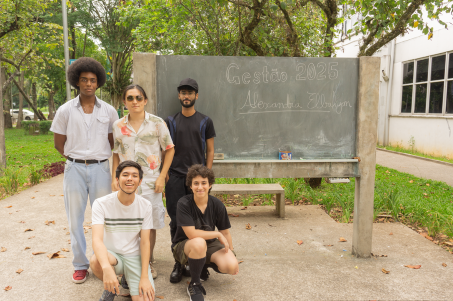
\includegraphics[width=0.6\linewidth]{textos//img/gestao_2025.png}
    \legendaFigura{1.2}{\textit{
    Foto com alguns membros da gestão Alexandra Elbakyan 2025
    \legendaFiguraQuebraLinha
    Em pé, da esquerda para direita: Otávio Fonseca, Link Zhang, Gabriel Marques
    \legendaFiguraQuebraLinha
    Agachado, da esquerda para direita: Eduardo Yukio, Nicolas Miguel
    }}
\end{figure}

\end{adjustwidth}